\lecture{7}{2025-03-11}{Entropy and algorithm}{}
\begin{parag}{Experience little play}
    \begin{itemize}
        \item Think of something
        \item Ask yes or no question
        \item Find the answer
    \end{itemize}
    the game was called twenty questions in old U.S tv. We want to use entropy to understand this game.
\end{parag}
\begin{parag}{Last Week}
\begin{align*}
    H_D(X) = H_D(P) - -\sum_x p(x) \log_D p(x)
\end{align*}

We also saw those two bounds:
\begin{align*}
    0 \leq H_D(X) \leq \log_D \mid  \mathcal{A} \mid
\end{align*}
Information is always about option, more options you have, more information (the first way to introduce \textit{"entropy"})\\
We also saw:
\begin{align*}
    H(X \mid  Y = y) = - \sum_x p(x \mid  y) \log_Dp(x \mid  y)\\
    H(X \mid  Y = y) = - \sum_y \dots
\end{align*}
And we also saw that on average:
\begin{align*}
    H(X \mid  Y) \leq H(X) \\
    H(X \mid  Y, Z) \leq H(X \mid  Y) \leq H(X)
\end{align*}

We also saw the chain rule:
    \begin{align*}
       H(S_1, S_2, S_3, S_4) \\
       = H(S_2, S_4, S_1, S_3)
    \end{align*}
    The order in entropy doesn't matter,
    \begin{align*}
        = H(S_1) + H(S_2 \mid  S_1) + H(S_3 \mid  S_1, S_2) + H(S_4 \mid  S_1, S_2, S_3)
    \end{align*}
    An intresting way to use this, is if we combine the inequalities and the chain rule. The equality on the right sight is true if and only if $X$ and $Y$ are independent. there fore:
    \begin{align*}
        H(S_1, S_2, S_3, S_4) = H(S_1) + H(S_2) + H(S_3) + H(S_4)
    \end{align*}
    this equality is true if and only if $S_1, S_2, S_3, S_4$ are independent.
    
\end{parag}


\begin{parag}{The 20 question problem}
    Let $X$ be a random variable. What is the minimum number of "yes/no" question needed to identify $X$?, which question should be asked.
\end{parag}
\begin{parag}{Solution}
    Let us consider a binary code $ \Gamma$ for $X \in \mathcal{X}$
    \\
    Once $ \Gamma$ is fixed, we know $x \in \mathcal{X}$ if and only if we know the codeword $ \Gamma(x)$. The strategy consists in asking the $i$th question so as to obtein the $i$th bit of the codword $ \Gamma(x)$.
    \\
    The expected number of question $L(X, \Gamma)$, which is minimized if $ \Gamma$ is the encoding map of Huffman code

    \begin{subparag}{Example}
        Suppose that we know that $ \mathcal{X} = \{ $ cat, dog, pony$\}$, with:
        \begin{align*}
            p(cat) = \frac{1}{2}\\
            p(dog) = \frac{1}{4} \\
            p(pony) = \frac{1}{4}
        \end{align*}
        We want to make it the best way, the question we should ask is:
        \begin{itemize}
            \item is the animal a cat?

        \end{itemize}
       
        \begin{center}
            \begin{tabular}{cccccc}
                $X$ & a & b & c & d & e 
           \hline

        \end{tabular}
        \end{center}
        
        
    \end{subparag}
    We then do a Huffman tree:
    \begin{center}
        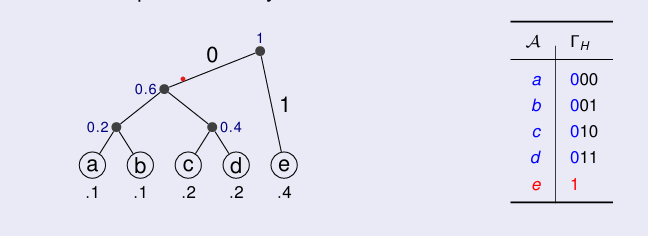
\includegraphics[0.7]{12025-03-11.png}
    \end{center}
    We know here that this, will be optimal
\end{parag}
\begin{parag}{Optimality}
    We have seen that a prefix free code for $X \in \mathcal{X}$ leads to a querying strategy to find the realization of $X$.
    \\
    Similarly, a deterministic querying strategy leads to a binary prefix-free code for $X$. Here is why:
    \begin{itemize}
        \item Before the first question we know that $x \in \mathcal{X}$
        \item Without loss of generality, the first question can be formulated in terms of "is $x \in \mathcal{A}$"? for some $ \mathcal{A} \subset \mathcal{X}$, (The choice of $ \mathcal{A}$ is determined from the strategy, that we fix once and for all)
        \item Is the answer is YES, the we know that $x \in \mathcal{A} \subset \mathcal{X}$. Otherwise $x \in A^c \subset \mathcal{X}$. Either way we have reduced the size of the set that contains $x$.
        \item We continue asking similar questions until the value of $x$ is fully determined, the we stop.
    \end{itemize}
    Here, the sequence of Yes or no answers is a binary codeword associated to $x$. The code obtained when we consider all possible values of $x$ is a binary prefix-free code. Since the tree is prefix free, its averag codeword-length cannot be smaller than that of a Huffman code.
\end{parag}

\begin{parag}{Sorting via pairwise comparisons}
    Given an \important{unsorted} List with $n$ elements.
    \\
    For example $l = [c, a, b]$ with $n = 3$
    \\
    \textbf{Repeat:}
    \begin{enumerate}
       \item Select two position $1 \leq i \leq j \leq n$
       \item Compare and swap:
           \begin{itemize}
               \item If $x_i > x_j$
               \item Then swap elements $ x_i \iff x_j$
               \item Else do nothing
           \end{itemize}
    \end{enumerate}
    One way to understands how it works:
\begin{center}
    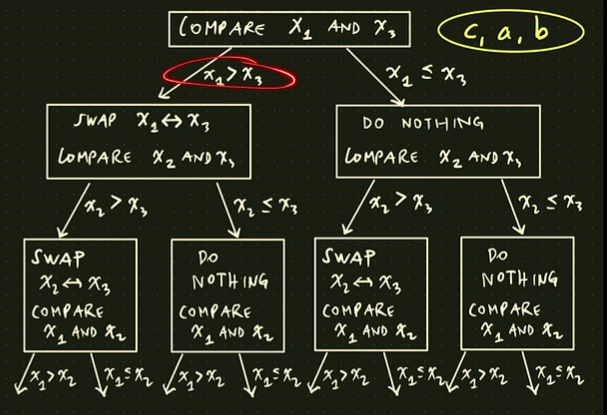
\includegraphics[scale=0.7]{22025-03-11.png}
\end{center}
The first observation:\\
The sequence of pairwise comparisons must identify the exact order of the unsorted list.
\\
The second observation:\\
The sequence of pairwise comparisons in a uniquely decodable (actually, prefix-free) binary code for $x$.\\
There fore, we must have:
\begin{align*}
    \mathbb{E}[ \text{number of comparisons}] \geq H_2(X)
\end{align*}
However what is the $X$? We see it as a random variable because we don't really know what the unsorted list is.\\
For example $n = 3$ we have $ \mathcal{X} = \{ abc, acb, bac, bca, cab, cba\}$ where $ \mathcal{X}$ is the set of all permutations.
\\
However what is $p(x)$? Here, we want to talk  about our algorithm working for all $p(x)$.
\\
\begin{align*}
    E &\geq max_{p(x)}H_2(X) = \log_2 \mid \mathcal{X} \mid \\
    &= \log_2 n!
\end{align*}
We already know a bounds on factorial:
\begin{align*}
    \frac{n^n}{e^{n-1}} \leq n! \leq \frac{n^{n+1}}{e^{n-1}}
\end{align*}

Therefore:
\begin{align*}
    H_2(x) &\approx \log_2 \frac{n^n}{e^{n-1}} \\
           &= n \log_2n - (n-1)\log_2 e
\end{align*}
Which is \textit{"dominated"} by $n\log_2 n$

\end{parag}

\begin{parag}{Billard Balls}
    There are 14 billards balls numbered as shown:
\begin{center}
    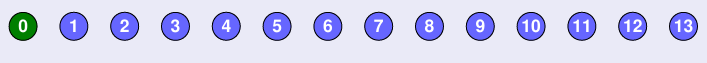
\includegraphics[scale=0.6]{32025-03-11.png}
\end{center}
Among balls $1-13$, at most one \textbf{could} be heavier/lighter than the others. What is the minimum number of weightings to simultaneously determine:
\begin{itemize}
    \item If one ball is different
    \item if there is such a ball which one, 
        \item And whether the different ball is heavier/lighter
\end{itemize}
Here we want to use entropy to solve this problem. The goal here is to associated the number of weightings to code. The goal is to see it as a tree.
\begin{center}
    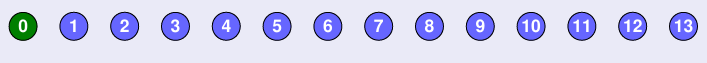
\includegraphics[scale=0.5]{32025-03-11.png}
\end{center}
The steps of picking two sets is \textit{"mandatory"} we have to pick two sets in order to compare something, and in order to compare something, you have to compare something...\\
From this comparisons, there will be three possibilities. with three possibilites, We are specifying a Ternary code. 
%\begin{framedremark}
 %   A remark during the course was:
  %  \begin{center}
    %    \textit{"Why can't we use binary, where we take the two inequalities together and the not equal alone?}
   % \end{center}
    The issue here is that we are losing information, yes we only get a binary tree however we wouldn't be able to have the same amount of information as with  a ternary tree. \\
    What we are saying here is, with any strategy to solve this problem \important{can} be written in this way. Hence we can read this tree as a ternary code.
%\end{framedremark}
\begin{subparag}{But a code for \important{What}?}
    What are we finding with this code?\\
    A code for $X$:
    \begin{itemize}
        \item $X = 0$: all balls are equals
        \item $X = +1$: ball $1$ is heavier
        \item $\vdots$ 
        \item $X = +13$ ball $13$ is heavier
        \item $X = -1$ balle $1$ is lighter
        \item $\vdots$
        \item $X = -13$ ball $13$ is lighter
    \end{itemize}
    Then we know that $ \mid \mathcal{X} \mid = 27$. This is one way to answers those question.
    \begin{enumerate}
        \item If $X = 0$ or not (then there is or not a different ball)
        \item Then  $ \mid X \mid $ gives us the information
        \item the sign of $X$ if the ball is heavier or lighter
    \end{enumerate}
    \textbf{Observation}
    The number of weighings  is equal to the length of the ternary codeword
\end{subparag}
Then:
\begin{theoreme}
    \begin{align*}
        \mathbb{E}[ \text{number of weighings}] \geq H_3(X)
    \end{align*}
\end{theoreme}
It has to be three by the way the problem is stated. The code is ternary \important{Therefore} the base for the entropy is $3$.\\
Moreover, our strategy must work \important{irrespective} of the probability distribution of $X$.
\\
We can also see:
\begin{theoreme}
    \begin{align*}
        \mathbb{E}[ \text{number of weighings}] \geq  \text{max}_{p(x)}(H_3(X))
    \end{align*}
\end{theoreme}
Where in our example gives us:
\begin{align*}
    \log_3 27 = 3
\end{align*}
\begin{framedremark}
    It doesn't need the be an integer it is only the professor that choose on purpose to make it clean
\end{framedremark}
\begin{subparag}{But does there indeed exists such a code}
    \textbf{FACT}:
    \begin{center}
        \important{Entropy} does \important{not} guarantee the existence of such a strategy
    \end{center}
   Entropy serves as a lower bound and \important{not} the best way to do it.  
\end{subparag}
    But can what if? \\
    Let us suppose it exists! Then entropy tells us a few basic facts.
\end{parag}
\begin{parag}{Fact 1}

         \important{if} $3$ weighings $S_1, S_2, S_3$ uniquely specify $X$, Then we \important{must have}:
            \begin{align*}
                H_3(X) = H_3(S_1, S_2, S_3)
            \end{align*} 
    
            \begin{subparag}{Proof}
                \begin{align*}
                    H(X, S_1, S_2, S_3) &= H(X) + \overbrace{H(S_1, S_2, S_3 \mid  X)}^{=0} \\
                                        &= H(S_1, S_2, S_3) + \overbrace{H(X \mid  S_1, S_2, S_3)}^{=0} \\
                \end{align*}
               It is true because if we know $S_1, S_2, S_3$ then we know all $X$ then the entropy of $0$. \\
               For $H(X \mid  S_1, S_2, S_3)$, because $S_1, S_2, S_3$ uniquely specify $X$ then knowing them implies that this entropy is $o$.
                
            \end{subparag}
  
\end{parag}


\begin{parag}{Fact 2}
    \important{If} 3 weighings $S_1, S_2, S_3$ uniquely specify $X$, then we must have:
    \begin{itemize}
        \item $S_1, S_2, S_3$ uniformly distributed
        \item $S_1, S_2, S_3$ independent
    \end{itemize}

    \begin{subparag}{Proof}
        \begin{align*}
            H_3(S_1, S_2, S_3) &= 3
        \end{align*}
        This is a \textit{must}.\\
        But also:
        \begin{align*}
            H_3(S_1) + H(S_2 \mid  S_1) + H(S_3 \mid S_1, S_2) \leq H_3(S_1) + H(S_2) + H(S_3) \\
            \leq \log_3 3 + \log_3 3 + \log_3 3
        \end{align*}
        Where it is an equality if and only if the distribution is uniform and independent.
        
        
    \end{subparag}
    
   
\end{parag}
\begin{parag}{Example}


Let's see how to actually find a way to ask those question:
\begin{center}
    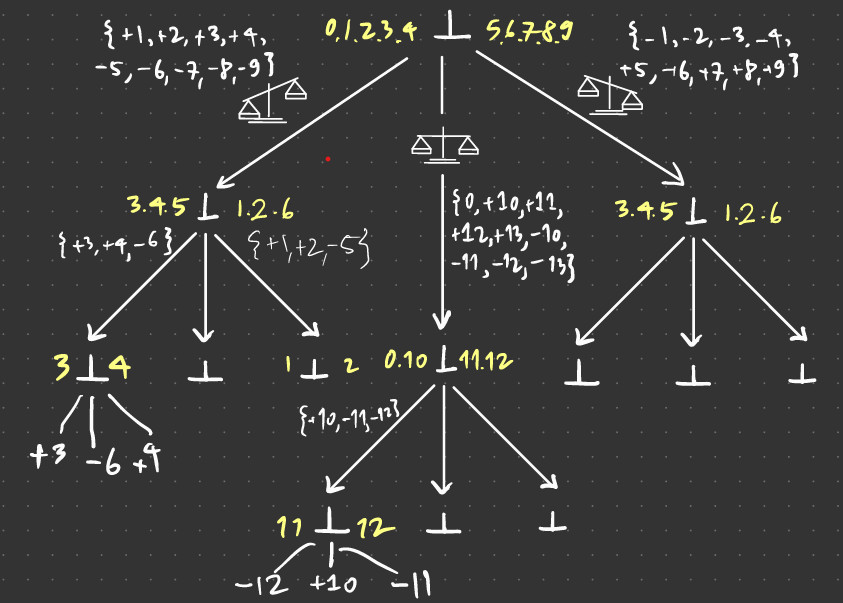
\includegraphics[scale=0.7]{52025-03-11.png}
\end{center}


\end{parag}
